\documentclass[12pt]{article}
\renewcommand{\familydefault}{\sfdefault}
\usepackage{csvsimple}
\usepackage{rotating}
\usepackage{graphicx}
\usepackage{hyperref}
\parindent=0pt
\parskip=5 pt
\setlength{\textwidth=7in}
\setlength{\oddsidemargin=-.25 in}
\setlength{\topmargin=0 in}
\setlength{\textheight=8.5 in}
%\usepackage{draftwatermark}
%\SetWatermarkText{Draft}
%\SetWatermarkScale{5}
\title{DUNE Offline Computing Model Calculations for 2024}
\author{H. Schellman for the Computing Consortium}
\date{\today -- version 1}



\newcommand{\hrefII}[1]{\href{#1}{#1}}

\newcommand{\ThisYear}{2024}
\newcommand{\CPUFNAL}{30.2}
\newcommand{\CPUCERN}{7.5}
\newcommand{\CPUGlobal}{37.7}
\newcommand{\CPUTotal}{75.4}
\newcommand{\CORESFNAL}{2742}
\newcommand{\CORESCERN}{686}
\newcommand{\CORESGlobal}{3428}
\newcommand{\CORESTotal}{6856}
\newcommand{\DISKFNAL}{9.5}
\newcommand{\DISKCERN}{4.7}
\newcommand{\DISKGlobal}{8.0}
\newcommand{\DISKTotal}{22.2}
\newcommand{\TAPEFNAL}{32.3}
\newcommand{\TAPECERN}{7.7}
\newcommand{\TAPEGlobal}{0.0}
\newcommand{\TAPETotal}{40.0}

\begin{document}


\makeatletter
\csvset{
  autotabularright/.style={
    file=#1,
    after head=\csv@pretable\begin{tabular}{|*{\csv@columncount}{r|}}\csv@tablehead,
    table head=\hline\csvlinetotablerow\\\hline,
    late after line=\\,
    table foot=\\\hline,
    late after last line=\csv@tablefoot\end{tabular}\csv@posttable,
    command=\csvlinetotablerow},
}
\makeatother
\newcommand{\csvautotabularright}[2][]{\csvloop{autotabularright={#2},#1}}

\maketitle



\section{Introduction}

This is an annual projection for DUNE CPU and storage needs intended for use at the Computing Contributions Board meeting in February 2024. It projects needs for \ThisYear\ to 2028. 

The overall computing model  and 2023 projections for DUNE were described in chapters 6-13 of the recent (Oct. 2022) DUNE Conceptual Design Report \cite{DUNE:2022fcw}.   This document provides updates on resource needs for 2024-2025. 

The \ThisYear\ projection is done using codes at: \href{https://github.com/DUNE/CCB-data/tree/CCB-Feb24/Numbers-2024/}{https://github.com/DUNE/CCB-data/tree/CCB-Feb24/Numbers-2024/} from parameters stored in a json and csv file. We use CPU and storage sizes derived from protoDUNE and simulation experience and apply them to projected numbers of events from the various DUNE detectors. 

This note summarizes pledges, usage and projected need for the CCB.

{\bf One Line Executive Summary:} Because the 2023 request assumed ProtoDUNE-2 running in 2023, the requests for 2024 are similar to the 2023 requests.





Changes since the last report \cite{CCB2023Report, CCB2023Minutes} include:

\begin{itemize}
\item Delay in the start of ProtoDUNE-2 running at CERN until mid-2024. This moves the need for storage/CPU into mid 2024. As the 2023 estimates were made assuming a 2023 run, most of the necessary resources are already in place. 
%\item Use of memory-weighted-core time instead of wall-time as our codes often require more memory than is available on a single core.  This means that our jobs sometimes need to reserve more than one core for a single process. This motivates the introduction of a memory-weighted wall-time unit for contributions  as different sites will  need to provide different amounts of wall-time to perform the same processing. 
\item Removal of the memory weighted core concept as it caused too much confusion and most available cores now have more than 2000 MB available. 
\item Switch to HS23-Years as opposed to Core-Years as the main CPU reporting system.
\item Revisions to near-term requests based on the 2023 experience including a hold on tape requests from the collaboration during protoDUNE activities. 
%\item Simulation disk copies continue to be reduced from 2 to 1.5 to fit within a reasonable profile.  If more disk becomes available we can restore more simulation copies.  
\item Changes to splits (Table \ref{tab:division}) between regions in disk and CPU provision. 
%\item A change in future tape requests to reflect the greater accessibility of tape archives at CERN and FNAL relative to other sites. 
\end{itemize}

\section{Model Summary}

Resource requests are based on a processing and storage model that separated different phases of the detectors and includes 4 classifications of activity.

\begin{itemize}
\item Data - described by number of events, CPU time/event, storage/event
\item Simulation - described by number of events,  CPU time/event, storage/event
\item Test - described by PB of storage, assumed not to consume large amounts of CPU
\item Analysis - described by a scaling factor relative to Reconstruction and Simulation CPU.
\end{itemize}

 Table \ref{tab:detectors} summarizes the detectors and their abbreviations. 

\begin{table}[h]
\begin{centering}
  \begin{tabular}{|l|l|l|}
     \hline
    Abbrev. & Detector & Running time\\
    \hline
    PDSP & ProtoDUNE Single Phase & 2018-2021\\
    PDDP & ProtoDUNE Dual Phase & 2018-2021\\
    PDHD & ProtoDUNE-2 Horizonal Drift & 2024-2026\\
    PDVD & ProtoDUNE-2 Vertical Drift & 2024-2026\\
    2x2& Prototype NDLAr Detector & 2024-2026\\
    HD & Far Detector Horizonal Drift & 2028-\\
    VD & Far Detector Vertical Drift & 2028-\\
    NDLAr + TMS & Near Detector Liquid Argon + Muon System & 2030-\\
    SAND & On Axis Near Detector & 2030- \\
     \hline
     \end{tabular}
       \caption{Detector descriptions.}\label{tab:detectors}
  \end{centering}
   
     \end{table}


These inputs are then used to calculate storage and CPU needs. 

Disk storage policies are designed to optimize access and minimize CPU inefficiencies due to network transfer speeds.  In particular, all recent data samples are planned to have at least one disk copy to avoid the need to access tape.  As raw data processing is not I/O bound, one disk copy has been found to be sufficient.  Analysis of reconstructed samples is I/O bound so multiple copies located closer to CPU are desirable. 

Each type of data has a storage retention policy which includes lifetimes on disk and tape and number of copies on disk and tape.  For example, raw data has a very long tape retention policy and 2 tape copies, with a 1 year stay of 1 copy on disk.   Recent simulated and reconstructed data samples typically have 1 tape copy, 2 disk copies and disk retention times of 1.5-2 years to allow fast analysis.   We assume one processing campaign per year, with all real data reprocessed each campaign.   Simulation is assumed to be redone as well but older samples are not reprocessed.  An extended retention time after the end of data taking for the last version of sim/reco is added to allow for extended data analysis. 

The model currently does not include any disk headroom allowance for data movement.  This will be added in the 2025 version of the model. 

CPU calculations are now made in HS23 units, with results from  2023 reported in both Core and HS23 units for reference.  Calculations for the protoDUNE's and DUNE far detector are based on existing reconstruction and simulation experience.  We have much less experience with Near Detector codes so those estimates are less accurate.

We assume protoDUNE running in 2024-2025 with startup of DUNE FD commissioning in 2027 (Test stream) and data taking in 2029. 



\begin{table}[h]
\begin{centering}
%\caption{Division between FNAL/CERN/Global for storage until 2027}
%{\bf Tape}
%\begin{tabular}{|rrrr|}
%\hline
% &FNAL&CERN & Global \\
% \hline
%Raw:&  0.5&  0.5&  0.0\\
%Sim:& 1.0&   0.0&   0.0\\ 
%Reco-Data:& 1.0&   0.0&   0.0\\
%Test: &  0.5&   0.5&  0.0\\
%
% \hline
%  \end{tabular}

 %  {\bf Disk and CPU splits}
     \begin{tabular}{|ll|rrr|}
     \hline
 &&FNAL:&CERN & Global \\
 \hline
 {\bf Disk} &&&&\\
 &Raw&   0.50&   0.50&  0.00\\ 
 &Sim: & 0.40&  0.10&  0.50\\
 &Reco-Data: &  0.40&   0.10&  0.50\\ 
 &Test: &  0.50& 0.50&   0.00\\
  \hline
{\bf Tape} &&&&\\
  &Raw:&   0.50&   0.50&  0.00\\ 
  &Rest"&  1.00 & 0.00 & 0.00\\
  \hline
{\bf CPU} &&&&\\
  &All: & 0.40& 0.10&0.50\\
  \hline
   \end{tabular}
  \caption{Proposed division between FNAL/CERN/Global for storage and CPU in the near term, until $\sim$2028, when FD replaces ProtoDUNE as the primary source of experimental data.  The tape division is not yet finalized as we work on integration of Global tape archives. In the long run, Global sites are expected to take over some of the tape provision currently provided by CERN. }

   \label{tab:division}
   \end{centering}
   \end{table}


\section{Pledge Requests}

Pledge requests for 2024 are similar to  those for 2023. Similar because  the impacts of ProtoDUNE running were already included in the 2023 request.

These  pledge requests include only general resources available to the DUNE collaboration, not the additional local resources available to collaborators at their own institutions.  

The near-term request does not include much Near Detector simulation.   That is currently being done via special allocations at NERSC and ANL and not yet included in our accounting.   

The model for proposed pledges for \ThisYear\ is detailed  in sections: Disk(\ref{sec:diskresult}), Tape(\ref{sec:taperesult}) and CPU(\ref{sec:cpuresult}) below.   A summary of requests and actual use for 2023 is shown in Table \ref{tab:summary2023} and the requests for \ThisYear\ are shown in Table \ref{tab:summary2024} 

\begin{table}[h]
\begin{centering}

\begin{tabular}{|ll|rr|rr|rr|}
\hline
 	&&	Disk (PB)	&	Actual	&	Tape(PB)	& Actual (PB)&CPU (Core-years)&Actual\\
	\hline
{\bf Model}	&&	25.80	&	--	&	45.5	&	-- & 15,169 & --	\\
\hline
{\bf Request}	&&		&		&		&	&	&\\
&FNAL	&	7.80	&	9.80&	36.2	& 27.1&	3,792& 2,844	\\
&CERN	&	2.60	&	4.02	&	9.2	& 5.7  &3,792	& 140\\
&Global	&	15.40	&	9.76	&	0.1	&  0.1 &	7,585 &1, 524\\
\hline
&{\bf Total}	&	25.80	& 23.58		&	45.5	& 32.9 & 15,169 	 & 4,515\\
\hline
\end{tabular}

\caption{Requests and actual usage from the previous year (2023).  CPU and disk utilization were low due to the delay in ProtoDUNE running. Table \ref{tab:RSEUsage}  shows the details of disk use by site.  CPU usage is detailed in  Table \ref{tab:CPUCores}. In this table  CPU is in units of unweighted core-years as that was the metric used prior to 2024.   }\label{tab:summary2023}
\end{centering}

\end{table}

\begin{table}[h]
\begin{centering}

\begin{tabular}{|llr|r|r|r|}
\hline
 	&&	Disk (PB)	&		Tape(PB)	&	CPU (kHS23-years)	 & CPU (Core-years)\\
	\hline
{\bf Model}	&&	\DISKTotal	&		\TAPETotal	&	\CPUTotal	& \CORESTotal\\
\hline
{\bf Request}	&&		 		&		&		\\
&FNAL	&	\DISKFNAL&	 	\TAPEFNAL	&	\CPUFNAL & \CORESFNAL	\\
&CERN	&	\DISKCERN	&	 	\TAPECERN&	\CPUCERN & \CORESCERN	\\
&Global	&	\DISKGlobal	&	 	--	&	\CPUGlobal   &\CORESGlobal\\
\hline
&{\bf Total}	&	\DISKTotal	&	 	\TAPETotal	&	\CPUTotal	 & \CORESTotal\\
\hline
\end{tabular}

\caption{Requests for 2024.  The disk requests reflect the different data types and the proposed splits from Table \ref{tab:division}.  They do not include the normal headroom of 5-10\%.  Tape pledges reflect the dominant use of CERN and FNAL for archival storage of data.  CPU pledges are in units of kHS23-years with Core-years provided for comparison to 2023.    }\label{tab:summary2024}
\end{centering}

\end{table}



\clearpage

\section{Supporting Materials}

Generally, raw data are stored on tape at both CERN and FNAL.  Simulation and reconstructed data  have one tape copy at Fermilab and recent reconstructed and simulated samples have one (or two) disk copies with one at Fermilab and one in Europe.  %Appendix \ref{storage} gives details on the size and types of data from the SAM data catalog.

CERN and FNAL have special responsibilities for archival data storage and for disk space for raw data while contributions from  other collaborating institutions are aggregated under the heading Global, which includes US sites outside of FNAL.  The proposed near-term  (until FD data taking) split between FNAL, CERN and Global contributions  is shown in Table \ref{tab:division}.  The pledges proposed here deviate slightly from those numbers with larger contributions from FNAL due to resources already in place. 


\subsection{Disk}
Table \ref{tab:RSEUsage} summarizes the disk utilization reported by sites via \cite{scotgrid}, supplemented by  rucio reports.   Some sites, notably TIFR, are not yet fully integrated so do not show up in the rucio reports.  %The contributions listed in Table \ref{tab:DiskPledges} sum the rucio and non-rucio disk known to be allocated to DUNE.

Figure \ref{fig:Cumulative-Disk}  summarize the cumulative disk needs and requests projected by our model. These numbers are used to generate the request for \ThisYear.  They are divided into the two host laboratories (CERN and FNAL) and Global, which includes contributions from the rest of the collaboration, including  BNL and NERSC in the US. 

Table \ref{tab:summary2023} summarized the pledges from previous years compared to the actual amounts allocated shown in Table \ref{tab:GlobalUsage} .   Because of the delay in ProtoDUNE running, disk that had been planned for ProtoDUNE data and simulation was not fully used.  
%\begin{table}[h]
%\centering\csvautotabularright{external/DUNERSEUSAGE-2022-11-14.csv}
%\caption{Summary  of DUNE disk areas known to rucio \cite{scotgrid}.  The CASTOR and FNAL Dcache areas are partially tape-backed and expandable. FNAL and CERN allocations are not provided by the reports but usage is.  }
%\label{tab:RSEUsage}
%\end{table}


\begin{table}[h]
%\begin{table}[h]
\centering
\csvautotabularright{external/StorageByCountry.csv}
\caption{Disk allocations and usage across countries at the end of 2023.    These numbers are derived from usage reports,  rucio reports and from cross-checks with individual sites on 2024-02-01.  The percentages are Used/Allocation. }
\label{tab:GlobalUsage}
%\end{table}
\end{table}

\begin{sidewaystable}[h]
%\begin{table}[h]
\centering
\csvautotabularright{external/RSEdata.csv}
\caption{Disk allocations and usage across sites.    These numbers are derived from usage reports,  rucio reports and from cross-checks with individual sites on 2024-02-01.  The percentages are Used/Allocation. }
\label{tab:RSEUsage}
%\end{table}
\end{sidewaystable}
%\end{document}

\begin{figure}[h]
\centering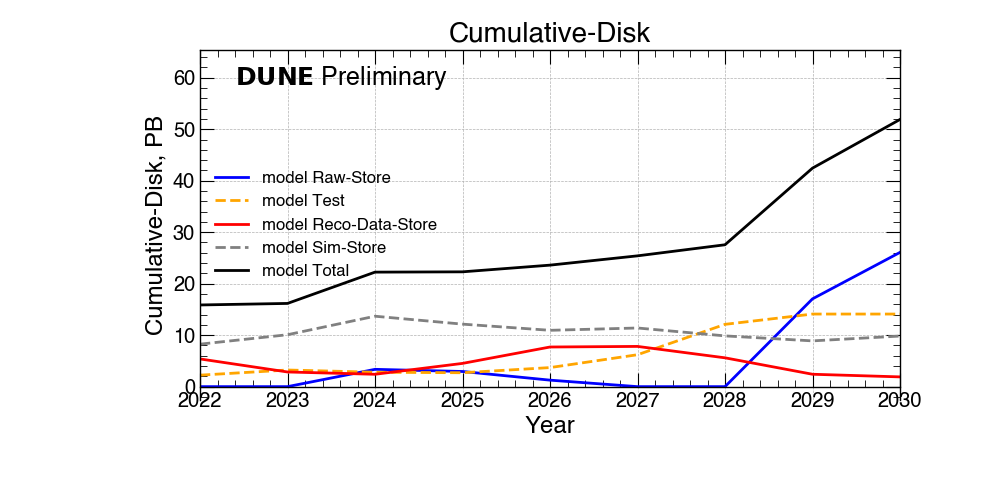
\includegraphics[height=0.5\textwidth]{NearTerm_2024-02-05-2030_noMWC/NearTerm_2024-02-05-2030_noMWC-Cumulative-Disk.png}
\csvautotabularright{NearTerm_2024-02-05-2030_noMWC/NearTerm_2024-02-05-2030_noMWC-Cumulative-Disk-Source.csv}
\csvautotabularright{NearTerm_2024-02-05-2030_noMWC/NearTerm_2024-02-05-2030_noMWC-Cumulative-Disk-Request.csv}
\caption{Cumulative Disk needs in PB. Includes data lifetimes.  The top table shows the source of the data while the bottom table  shows the proposed split using the fractions from Table \ref{tab:division} and a modified version which reflects the disk already in place at FNAL and CERN, thus reducing the Global request. }\label{fig:Cumulative-Disk}
\end{figure}




%\begin{table}[h]
%\centering\csvautotabularright{external/DiskResources-2021-2022-2023-2024-Details.csv}
%\caption{Summary of disk pledges, allocations and usage for 2021-2022 with model request for 2023.  This is based on the 2022 CCB tables which are available in indico  \cite{CCB2022,CCB2023}.  These numbers are derived from the rucio reports in Table \ref{tab:RSEUsage} and may not be complete.  }
%\label{tab:DiskPledges}
%\end{table}

\subsubsection{Request Summary}\label{sec:diskresult}
The total disk request for 2024 is \DISKTotal PB.  This is consistent with the current allocated space of 24.3 PB. Because 5-10\% headroom is needed, we request that the current allocated  24.3 PB be retained for 2024. 

\clearpage
\subsection{Tape}

\subsubsection{Current Status}

DUNE currently has $\sim$27.1 PB of data\cite{fnaltape} on tape at Fermilab and 5.7 PB of raw protoDUNE data  at CERN\cite{scotgrid}. 

\subsubsection{Model Projections}

Figure  \ref{fig:Cumulative-Tape}  summarizes the cumulative  tape needs projected by  the model. These numbers are used to generate the requests for 2024.  They are divided into the two host laboratories (CERN and FNAL). The UK and the IN2P3 have offered $\sim 3$ PB of tape archive  but it has not yet been smoothly integrated into our data flow.  We  therefore substantially reduce our request for  resources  at those sites to $\sim 100$ TB per site, to allow testing of integration, with an increased request anticipated future years. .

The increase in 2024-2025 is mainly storage of raw and processed  data from the upcoming runs of PDHD and PDVD.

The exact division between FNAL, CERN and Global once DUNE starts taking FD data in 2029 is not yet defined.  



\subsubsection{Current Status and Request}\label{sec:taperesult}
 We anticipate needing \TAPETotal\ PB of tape (an increase of 7 PB from 2023) to accommodate the ProtoDUNE run 2 data and increased simulation. 


\begin{figure}[h]
\centering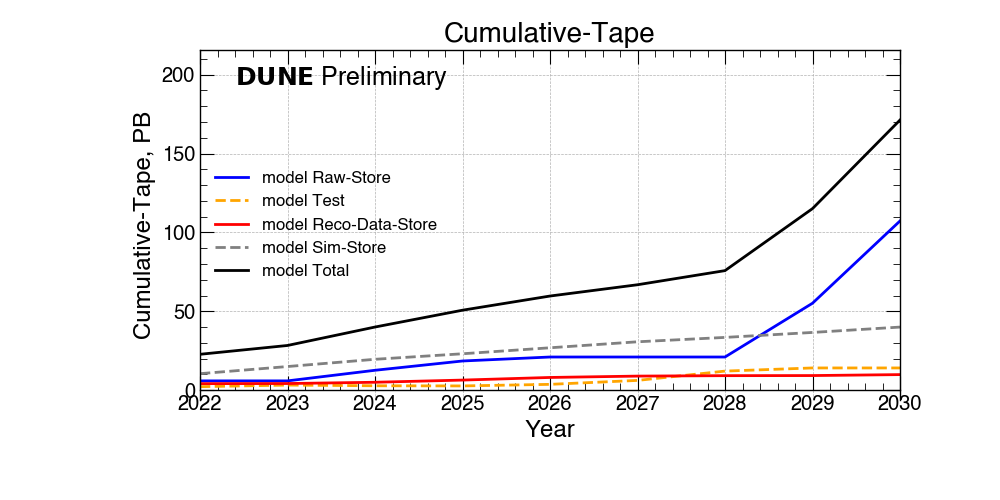
\includegraphics[height=0.4\textwidth]{NearTerm_2024-02-05-2030_noMWC/NearTerm_2024-02-05-2030_noMWC-Cumulative-Tape.png}

\csvautotabularright{NearTerm_2024-02-05-2030_noMWC/NearTerm_2024-02-05-2030_noMWC-Cumulative-Tape-Source.csv}
\csvautotabularright{NearTerm_2024-02-05-2030_noMWC/NearTerm_2024-02-05-2030_noMWC-Cumulative-Tape-Request.csv}
%\csvautotabularright{external/NearTerm_2024-02-05-2030_noMWC-Cumulative-Tape-Request.csv}
\caption{Cumulative Tape needs from the model in PB, includes data lifetimes.  The top table shows the origin of the data while the bottom table  shows the proposed split.  Global contributions are set low in \ThisYear\ and grow thereafter as more tape archives are integrated. The exact division between FNAL, CERN and Global once DUNE starts taking FD data in 2029 is not yet defined.  
 }\label{fig:Cumulative-Tape}
\end{figure}



\clearpage
\subsection{CPU }

\subsubsection{Current Status}
Tables \ref{tab:CPUCores} and \ref{tab:CPUusage} show the CPU used by country  in calendar 2023.  Due to the delay in ProtoDUNE running CPU use was dominated by code development and analysis of the older ProtoDUNE data.   Total CPU use was substantially lower than projected.
%Table \ref{tab:CPUUsage} shows pledges and utilization for 2021-2022 and the request for 2023.  

%DUNE differs from other HEP experiments in frequently requiring more memory/core than is available at particular sites.  For example an 8-slot pilot with 16 GB of available memory may only accommodate four reconstruction processes.   As a result, we make our requests in terms of memory-weighted-core wall time (MWC)  with the base memory being 2000 MB. This maps reasonably well to the memory weighted slot-time returned by HTCondor and the slot-time reported in EGI statistics.  Sites that offer more  (or less) than 2000 MB/core can scale their contributions up by the local memory/core.

\begin{table}[h]
\centering\csvautotabularright{external/Usage_CoreYears_2023-01-01-2023-12-31_ByCountry.csv}
\caption{CPU utilization in Core Years  for calendar 2023 divided by use case.  This is for comparison with the previous pledging system.    Production includes  official reconstruction and simulation. Analysis is user analysis of data.  MARS is beamline simulations performed at Fermilab.  NoMARS sums just Production and Analysis.  }
\label{tab:CPUCores}
\end{table}

\begin{table}[h]
\centering\csvautotabularright{external/Usage_kHS23-Yrs_2023-01-01-2023-12-31_ByCountry.csv}
\caption{CPU utilization in kHS23-Years for calendar 2023 divided by use case.   Production includes official reconstruction and simulation. Analysis is user analysis of data.  MARS is beamline simulations performed at Fermilab.  NoMARS sums just Production and Analysis. }
\label{tab:CPUusage}
\end{table}


\subsubsection{Model calculation}
The wall-time estimates in the model are created by estimating the number of simulated and raw events taken and then scaling by the measured CPU time per event on a gpvm corrected to wall-time by the estimated efficiency (default 70\%).  Each data type also has an additional "Analysis" factor of 0.5 to 1.0  to account for analysis after the original reconstruction.  

The numbers for PD and FD are based on substantial experience with the earlier ProtoDUNE runs and  large-scale simulation campaigns.  The numbers for ND are much more uncertain and await experience with  simulation and reconstruction of results from the 2x2 demonstrator which will run later in \ThisYear\ at Fermilab. The model shows ProtoDUNE dominating through the 2024-2025 runs and subsequent analysis period with  testing and simulation for the DUNE near and far detectors taking over circa 2028. 


 %and for a memory utilization factor that takes into account the differing memory needs for different applications. Here we assume that analysis takes 3000 MB, reconstruction takes 4000MB, and simulation takes 6000MB.  Contributions are then requested in units of MWC-time which is wall-time$\times$2000 MB units. 


%\begin{figure}[h]
%\centering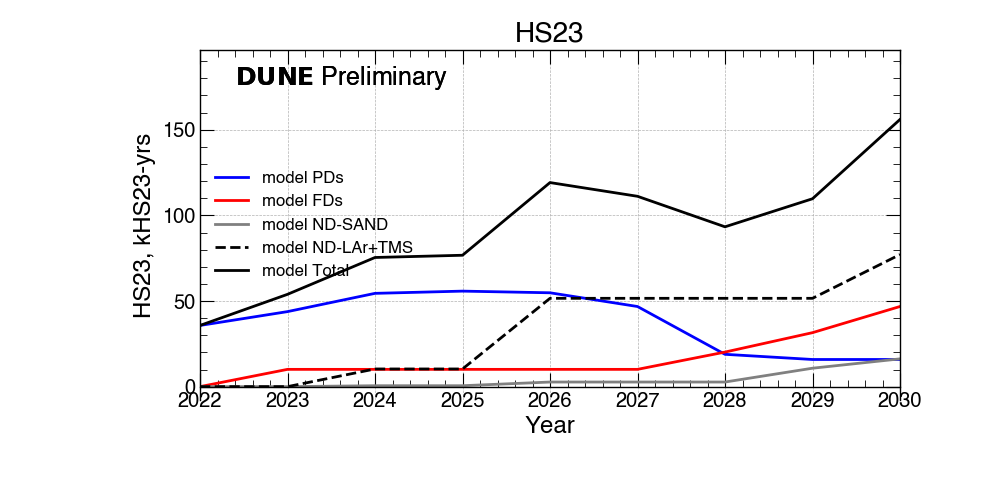
\includegraphics[height=0.4\textwidth]{NearTerm_2024-02-05-2030_noMWC/NearTerm_2024-02-05-2030_noMWC-HS23.png}
%\csvautotabularright{NearTerm_2024-02-05-2030_noMWC/NearTerm_2024-02-05-2030_noMWC-HS23.csv}  %had to fix so moved to external
%\caption{Proposed wall-time needs in number of 2000 MB HS23 (MWC-years). Memory-weighted  wall-time takes into account memory and efficiency.}\label{fig:HS23Main}
%\end{figure}

\begin{figure}[h]
\centering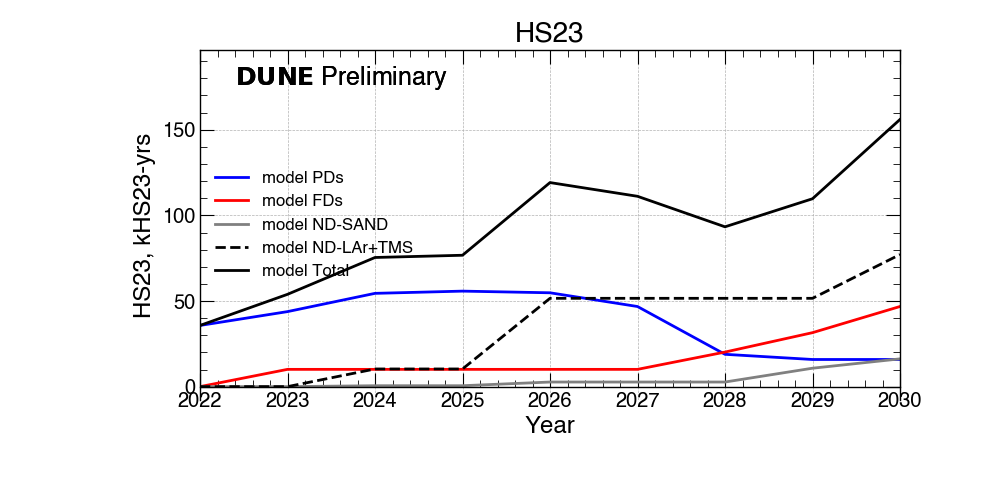
\includegraphics[height=0.4\textwidth]{NearTerm_2024-02-05-2030_noMWC/NearTerm_2024-02-05-2030_noMWC-HS23.png}
\csvautotabularright{NearTerm_2024-02-05-2030_noMWC/NearTerm_2024-02-05-2030_noMWC-HS23.csv}  %had to fix so moved to external
\caption{Model of CPU wall-time needs  through 2030 in  kHS23-yr units.  The top 4 lines show division by detector, the bottom 4 show the proposed division between FNAL, CERN and Global based on the fractions in Table \ref{tab:division}.}\label{fig:HS23Main}
\end{figure}


Figure   \ref{fig:HS23Main} shows the projected wall-time  (HS23-yrs) need projections through 2030.   They are divided into the two host laboratories (CERN and FNAL) and Global, which includes contributions from the rest of the collaboration, including OSG, BNL and NERSC in the US. 


%
%\subsection{Example of memory weighted pledges}
%An example of a  national pledge in MWC might be  1000 cores with 2GB available/core, 500 cores with 4 GB available/core and 100 cores with 8 GB available/core.  The MWC pledge would then be 
%
%\newcommand{\GB}{\hbox{GB}}
%
%\begin{eqnarray*} 1000\times2\GB/2\GB &+& \\ 500\times4\GB/2\GB &+&\\100\times8\GB/2\GB\\&&= 2400 \hbox{\ MWC units}\end{eqnarray*}.
%
%A pledge with cores with $<$ 2 GB would get partial MWC units per core. 
%
%The idea here is make the additional load of running large DUNE jobs transparent to sites, which either need to provide more than 2GB of memory/job or assign more cores than are actually used to a given job.  How a site makes and meets a pledge is up to the site management. Table \ref{tab:VOcard} summarizes the memory specifications from existing "VO" cards for the different experiments.  DUNE and LHCb currently are the only ones with a stated maximum $>$ 2048 MB.

%\subsection{CPU Requests}
%
%We request \CPUTotal\  kHS23-Years of computing for 2024 to support reconstruction, calibration and analysis of ProtoDUNE data and simulation studies for the future far and near detectors. 
%





%Table \ref{tab:CPUUsage} summarizes previous pledges\cite{CCB2023}. %and the measured usage  for 2021 and 2022 using FNAL's  HTCondor memory-weighted wall-time statistics\cite{fifemonDUNE}.  The  usage numbers for 2022 are Nov 2021 to Oct 2022. 

%Table \ref{tab:EIGSummary} summarizes the statistics for European sites from Nov 2021 to Oct 2022 derived from the EGI accounting\cite{EGI2022} which uses the number of cores allocated to a pilot.   If four 4000 MB reconstruction jobs were sent to an 8-core pilot on a system with 2000MB/core, this would be equivalent to using 8 MWC (memory-weighted wall-time units).   


%\begin{table}[h]
%\centering\csvautotabularright{external/CPUresources-2021-2022-2023-v3.csv}
%\caption{Summary  of DUNE wall-time pledges and contributions for 2021 and 2022.  The 2022 actual numbers are memory-weighted core-years.  Individual nations are listed and then merged (with US OSG) into a Global section.} 
%\label{tab:CPUUsage}
%\end{table}

%\begin{table}[h]
%\centering\csvautotabularright{external/EIG-2022.csv}
%\centering\csvautotabularright{external/EIG-2022-Global.csv}
%\caption{Summary  of DUNE slot-years used for European collaborators, Nov. 21 to Oct. 22, using the EGI accounting\cite{EGI2022}.  The top shows all sites with EGI records, the bottom shows the summed contributions. These numbers reflect multiple-core slot reservations to account for larger memory use and are similar to, but  generally higher than, the FNAL accounting numbers in the previous table.} \label{tab:EIGSummary}
%\end{table}
%
%\begin{table}[h]
%\centering
%\begin{tabular}{|l|l|l|}
%\hline
%Expt.&Max Memory& EGI VO Card\\
%\hline
%DUNE & 4000& \hrefII https://operations-portal.egi.eu/vo/view/voname/DUNE \\
%ATLAS & 2000& \hrefII https://operations-portal.egi.eu/vo/view/voname/atlas \\
%CMS & 2000& \hrefII https://operations-portal.egi.eu/vo/view/voname/cms \\
%LHCb & 4000& \hrefII https://operations-portal.egi.eu/vo/view/voname/lhcb \\
%ALICE& 2000& \hrefII https://operations-portal.egi.eu/vo/view/voname/alice \\
%BelleII&2048& \hrefII https://operations-portal.egi.eu/vo/view/voname/belle \\
%\hline
%\end{tabular}
%\caption{Maximum memory statements from the VO cards of major experiments.}
%\label{tab:VOcard}
%\end{table}
%

\subsubsection{CPU Request}\label{sec:cpuresult} The advent of ProtoDUNE-2 running in \ThisYear\ and ramp-up of simulation for the FD and ND will lead to somewhat increased needs for CPU resources.  For \ThisYear, we are requesting \CPUTotal\   kHS23-Yrs.
%\section{
%\section{Projected Disk and Tape needs by source and site}
\begin{figure}[h]
\centering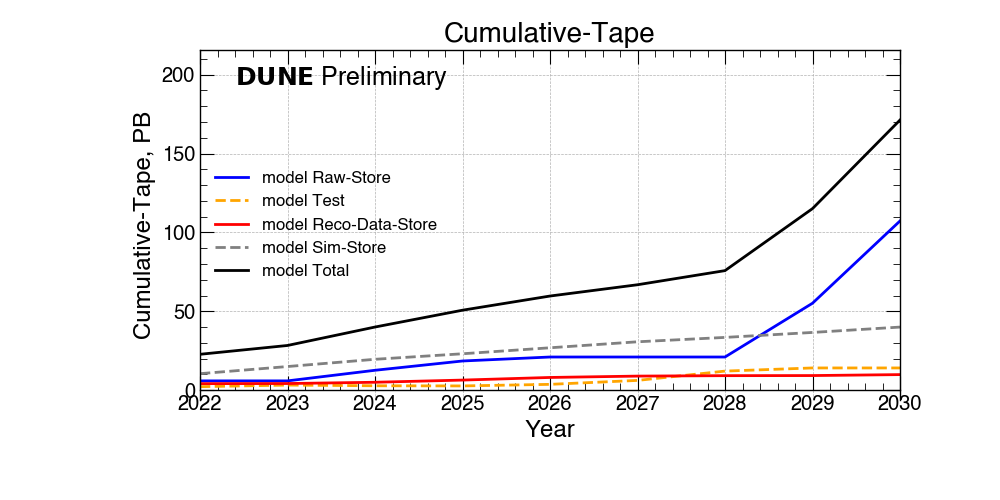
\includegraphics[height=0.4\textwidth]{NearTerm_2024-02-05-2030_noMWC/NearTerm_2024-02-05-2030_noMWC-Cumulative-Tape.png}
\csvautotabularright{NearTerm_2024-02-05-2030_noMWC/NearTerm_2024-02-05-2030_noMWC-Cumulative-Tape.csv}\caption{Cumulative Tape needs in PB. Includes multiple copies and data lifetimes. The top 4 lines show the source of the data while the last four propose responsibilities.}
\label{fig:Cumulative-Tape}
\end{figure}
\begin{figure}[h]
\centering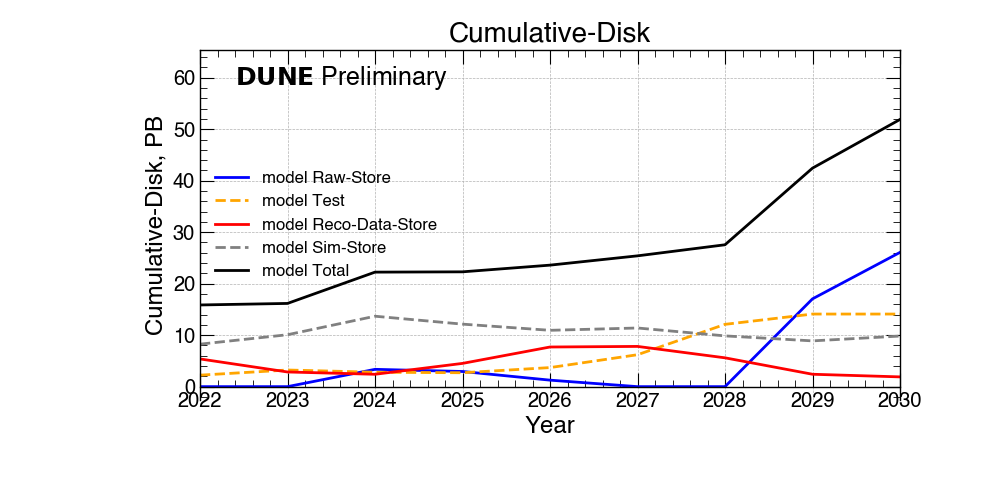
\includegraphics[height=0.4\textwidth]{NearTerm_2024-02-05-2030_noMWC/NearTerm_2024-02-05-2030_noMWC-Cumulative-Disk.png}
\csvautotabularright{NearTerm_2024-02-05-2030_noMWC/NearTerm_2024-02-05-2030_noMWC-Cumulative-Disk.csv}\caption{Cumulative Disk needs in PB. Includes multiple copies and data lifetimes. The top 4 lines show the source of the data while the last four propose responsibilities.}
\label{fig:Cumulative-Disk}
\end{figure}


%\sectionHS23{Model Assumptions}

\cleardoublepage
%\renewcommand{\bibname}{References}
\bibliographystyle{utphys} 
\bibliography{bib}
\clearpage
\appendix

%\section{Information about storage from SAM}\label{storage}
%
%This section provides information on the sizes of data samples known to the SAM data catalog as of Nov. 1, 2022.  If a file has multiple copies, that is not shown here.  Tables \ref{tab:MCinSAM} and \ref{tab:DataInSam} show the total across all streams and data tiers while table \ref{tab:LargestSizes} shows the distribution of the largest samples.  
%
%
%\begin{table}[h]
% \centering\csvautotabularright{external/mc.csv}
%\caption{Summary  of total simulation in SAM by detector type as of Nov 1, 2022.} 
%\label{tab:MCinSAM}
%\end{table}
%
%\begin{table}[h]
% \centering\csvautotabularright{external/detector.csv}
% \caption{Summary  of total detector data in SAM by detector type as of Nov 1, 2022.}
% \label{tab:DataInSam}
%\end{table}
%
%
%
%\begin{table}[h]
% \centering\csvautotabularright{external/TOPTYPES.csv}
%\caption{Classification of the largest data samples in SAM.  They are classified as detector(data) or mc, by the detector producing the data, by the stream (readout time) and by the data tier.  Some types, test and noise for example are archival only.  }
% \label{tab:LargestSizes}
%\end{table}
%\clearpage
\section{Model Details}

This appendix shows the parameters used in the model and plots of all the input and derived quantities as a function of time. 

Resource needs for reconstructed data for a given year are based on the number of events produced over the previous "Reprocess" years.   For ProtoDUNEs that is 2-4 years. 

Simulation resource needs are instead calculated based on a number of simulation events each year. The assumption is that new software versions imply resimulation.

Disk and tape lifetimes for different data types are specified as well as the desirable number of copies. 

The splits parameters make CERN responsible for raw data until 2027 with the collaboration taking over after that point. 

{\tt Detectors:} Detectors included in the calculation = {\tt ['SP', 'SP2', 'DP', 'PDVD', 'HD', 'VD', 'ND']} \\
{\tt Cap:} Cap on Raw data/year in PB = {\tt 30} \\
{\tt Base-Memory:} MB of memory per slot assumed as the average = {\tt 2000} \\
{\tt MaxYear:} Plot until year = {\tt 2027} \\
{\tt MinYear:} Plot starting with year = {\tt 2021} \\
{\tt Reprocess:} Number of years of data reprocessed when doing a new pass = {\tt {'SP': 3, 'DP': 2, 'SP2': 4, 'PDVD': 4, 'PDs': 3, 'VD': 100, 'HD': 100, 'FDs': 100, 'ND': 100, 'MARS': 1}} \\
{\tt PatternFraction:} Fraction of time taken in pattern recognition = {\tt {'SP': 0.7, 'SP2': 0.7, 'DP': 0.7, 'PDVD': 0.7, 'PDs': 0.7, 'HD': 0.1, 'VD': 0.1, 'FDs': 0.1, 'ND': 0.9, 'MARS': 0}} \\
{\tt TapeLifetimes:} Number of years kept on tape = {\tt {'Raw-Store': 100, 'Test': 0.5, 'Reco-Data-Store': 15, 'Sim-Store': 15}} \\
{\tt DiskLifetimes:} Number of years kept on disk = {\tt {'Raw-Store': 1, 'Test': 0.5, 'Reco-Data-Store': 2, 'Sim-Store': 2}} \\
{\tt TapeCopies:} Number of copies kept on tape = {\tt {'Raw-Store': 2, 'Test': 1, 'Reco-Data-Store': 1, 'Sim-Store': 1}} \\
{\tt DiskCopies:} Number of copies kept on disk = {\tt {'Raw-Store': 1, 'Test': 1, 'Reco-Data-Store': 2, 'Sim-Store': 1.5}} \\
{\tt PerYear:} Number of reprocessing done per year = {\tt {'Raw-Store': 1, 'Test': 1, 'Reco-Data-Store': 1, 'Sim-Store': 1, 'Events': 1, 'Sim-Events': 1, 'Reco-Data-CPU': 1, 'Sim-CPU': 1, 'Analysis': 1, 'Analysis-CPU': 1}} \\
{\tt Cores:} Description of cores, efficiency and speed relative to 2020 vintage = {\tt {'Efficiency': 0.7, '2020Units': 1}} \\
{\tt kHEPSPEC06PerCPU:} kHEPSPEC06 per core assumed = {\tt 0.011} \\
{\tt SplitsYear:} Year CERN no longer responsible for disk or tape = {\tt 2029} \\
{\tt SplitsEarly:} Division between FNAL/CERN/National for storage until SplitsYear = {\tt {'Tape': {'Raw-Store': {'FNAL': 0.5, 'CERN': 0.5, 'National': 0.0}, 'Sim-Store': {'FNAL': 1.0, 'CERN': 0.0, 'National': 0.0}, 'Reco-Data-Store': {'FNAL': 1.0, 'CERN': 0.0, 'National': 0.0}, 'Test': {'FNAL': 0.5, 'CERN': 0.5, 'National': 0.0}}, 'Disk': {'Raw-Store': {'FNAL': 0.5, 'CERN': 0.5, 'National': 0.0}, 'Sim-Store': {'FNAL': 0.4, 'CERN': 0.1, 'National': 0.5}, 'Reco-Data-Store': {'FNAL': 0.4, 'CERN': 0.1, 'National': 0.5}, 'Test': {'FNAL': 0.5, 'CERN': 0.5, 'National': 0.0}}, 'CPU': {'CPU': {'FNAL': 0.4, 'CERN': 0.1, 'National': 0.5}}}} \\
{\tt SplitsLater:} Division between FNAL/CERN/National for storage after SplitsYear = {\tt {'Tape': {'Raw-Store': {'FNAL': 0.5, 'CERN': 0.0, 'National': 0.5}, 'Sim-Store': {'FNAL': 0.5, 'CERN': 0.0, 'National': 0.5}, 'Reco-Data-Store': {'FNAL': 0.5, 'CERN': 0.0, 'National': 0.5}, 'Test': {'FNAL': 0.5, 'CERN': 0.0, 'National': 0.5}}, 'Disk': {'Raw-Store': {'FNAL': 1.0, 'CERN': 0.0, 'National': 0.0}, 'Sim-Store': {'FNAL': 0.25, 'CERN': 0.0, 'National': 0.75}, 'Reco-Data-Store': {'FNAL': 0.25, 'CERN': 0.0, 'National': 0.75}, 'Test': {'FNAL': 0.5, 'CERN': 0.0, 'National': 0.5}}, 'CPU': {'CPU': {'FNAL': 0.5, 'CERN': 0.0, 'National': 0.5}}}} \\
{\tt filename:} Input configuration file = {\tt MoreSim\_2023-01-31-2040.json} \\


\end{document}
%\end{document}
%https://tex.stackexchange.com/questions/292512/csvsimple-csvautotabular-and-csvautobooktabular-with-centered-columns-content
